\section{Tilstandsmaskin}
\thispagestyle{fancy}

Då \gls{IEC}-blokkene var ferdige, byrja vi på tilstandsmaskina som skulle styre sjølve \gls{SBR}-prosessen. 
Vi hadde allereie danna oss eit bilete, men kunne no byrje å nytte kunnskapen frå anleggets verkemåte
til å grovt fylle inn dei hendelsane og aksjonane som foregikk mellom tilstandane. 
Tilstandsmaskina er bygd opp av dei fem reaktorsekvensane som eksisterar i eit \gls{SBR}-anlegg.

Dette er ein enkel modell av korleis tilstandsmaskina er programmert, men gir eit godt innblikk i funksjonaliteten. \newline \newline \newline \newline \newline

\begin{figure}[htbp]
    \centering
    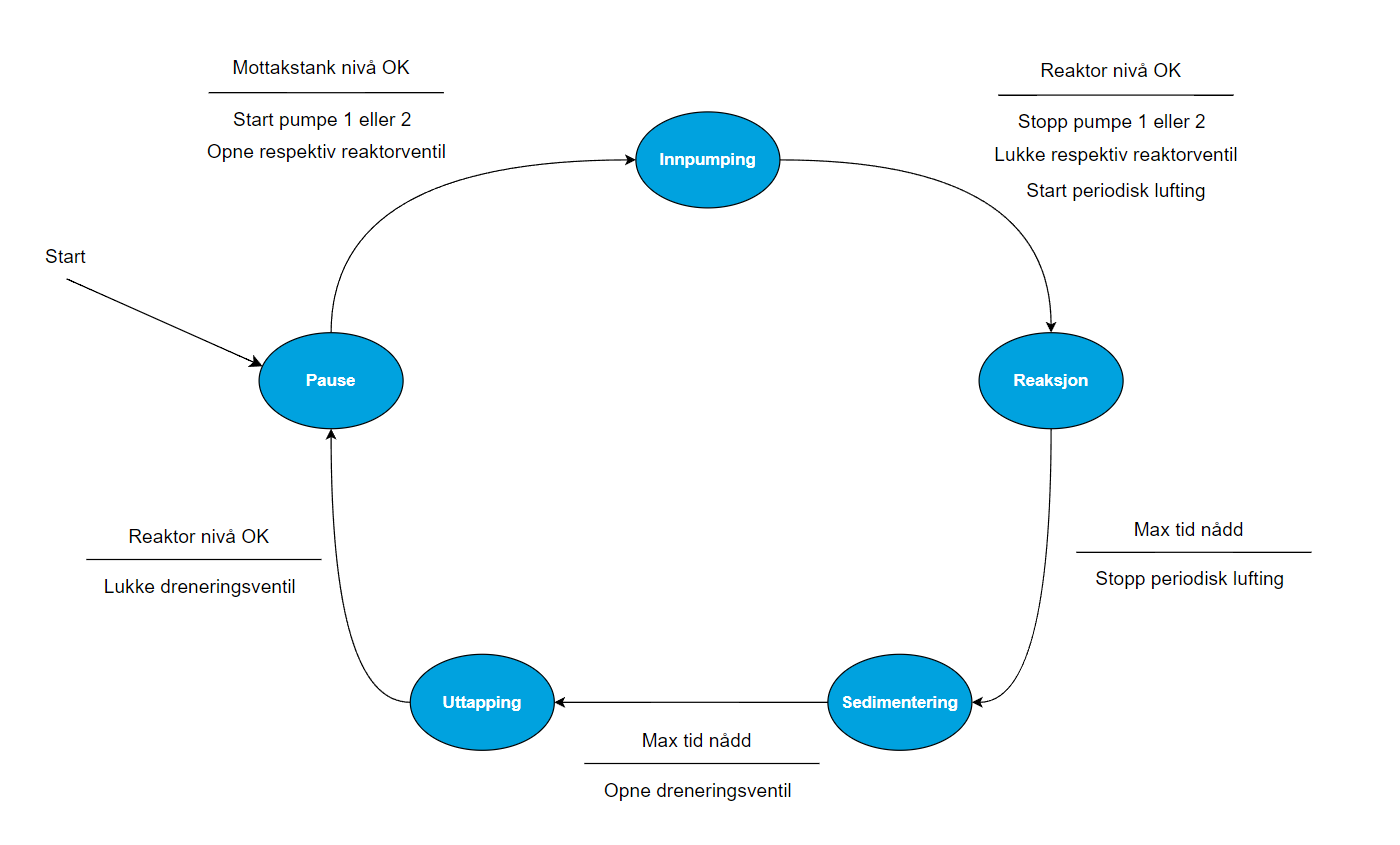
\includegraphics[width=1\textwidth]{Figurar/Simpel tilstandsmaskin.png}
    \caption{Enkel model av tilstandsmaskin}\label{fig:SimpelTilstandsmaskin}
\end{figure}


\newpage

I sjølve programmeringa av tilstandsmaskina blei den oppretta som ei eiga funksjonsblokk, noko som gav oss moglegheita å nytte blokka for begge reaktorane.
Tilstandsmaskina er laga med fem inngangar og seks utgangar, og baserer seg på ``switch/case'' logikk.

Tilstandsmaskina sender ut høg på den respektive utgangen som samsvarer med reaktortilstanden den er i. Dersom tilstandsmaskina får tilbake
høg på den respektive tilstandsinngangen avanserer tilstandsmaskina.
Det er også mogleg å hente ut aktiv tilstand ved hjelp av ein heiltallsverdi (1-5) \newline \newline \newline \newline

\begin{figure}[htbp]
    \centering
    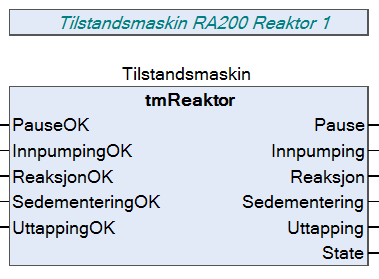
\includegraphics[width=0.6\textwidth]{Bilder/Tilstandsmaskin.png}
    \caption{Tilstandsmaskin implementert i programmet}\label{fig:TilstandsmaskinIProgram}
\end{figure}


